\حصہ{فشار سیال اور سیالی قوتیں}
فشار \عددی{p} سے مراد وہ قوت ہے جو اکائی رقبہ پر عمل کرتی ہو۔ یوں اگر رقبہ \عددی{S} پر قوت \عددی{F} عمل کرتی ہو تب فشار \عددی{p} درج ذیل ہو گا۔
\begin{align}\label{مساوات_تکمل_استعمال_فشار_اور_قوت}
p=\frac{F}{S}
\end{align}
\جزوحصہء{مستقل گہرائی پر سیال کی فشار اور قوت}
 شکل \حوالہ{شکل_تکمل_استعمال_فشار_سیال_تعریف} میں ساکن سیال کو ایک برتن میں دکھایا گیا ہے جہاں تلہ کا رقبہ \عددی{S}، سیال کی گہرائی \عددی{h} اور  سیال کی کثافت \عددی{\rho} ہے۔ یوں سیال کا حجم \عددی{Sh}،  کمیت \عددی{\rho Sh} اور وزن \عددی{g\rho Sh} ہو گا۔ سیال کے وزن کے برابر قوت \عددی{F=g\rho Sh} رقبہ \عددی{S} پر عمل کرے گی۔ یوں اکائی رقبہ پر قوت \عددی{g\rho h} ہو گی جس کو \اصطلاح{فشار}\فرہنگ{فشار}\حاشیہب{pressure}\فرہنگ{pressure} \عددی{p} یا \اصطلاح{دباو}\فرہنگ{دباو}  کہتے ہیں۔
\begin{align}\label{مساوات_تکمل_استعمال_فشار_سیال_الف}
p&=\rho g h
\end{align}
فشار کی اکائی  نیوٹن فی مربع میٹر \عددی{\si{\newton\per\meter\squared}} ہے۔ آپ نے دیکھا کہ سیال کی قیمت پر برتن کی صورت کا کوئی اثر نہیں پایا جاتا ہے۔

 مستقل گہرائی کے رقبہ پر درج ذیل قوت پایا جائے گا۔
\begin{align}
F=pS
\end{align}
%
\begin{figure}
\centering
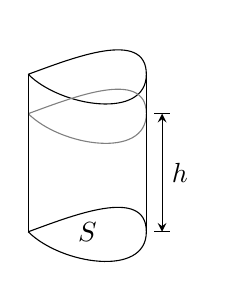
\begin{tikzpicture}[]
\pgfmathsetmacro{\h}{2}
\pgfmathsetmacro{\r}{1.5}
\draw(0,0)to [out=-45,in=-90] ++(\r,0) to [out=90,in=20]++(-\r,0);
\draw(0,\h)to [out=-45,in=-90] ++(\r,0) to [out=90,in=20]++(-\r,0);
\draw[gray](0,3/4*\h)to [out=-45,in=-90] ++(\r,0) to [out=90,in=20]++(-\r,0);
\draw(0,0)--++(0,\h)  (\r,0)--++(0,\h);
\draw(\r+0.1,0)--++(0.2,0)coordinate[pos=0.5](k);
\draw(\r+0.1,3/4*\h)--++(0.2,0);
\draw[stealth-stealth](k)--++(0,3/4*\h)node[pos=0.5,right]{$h$};
\draw(0.75,0)node[]{$S$};
\end{tikzpicture}
\caption{فشار سیال۔}
\label{شکل_تکمل_استعمال_فشار_سیال_تعریف}
\end{figure}

سیال میں \عددی{h} گہرائی پر کسی بھی رخ فشار کی قیمت  مساوات \حوالہ{مساوات_تکمل_استعمال_فشار_سیال_الف} دیتی ہے۔ یوں کسی بھی گہرائی پر افقی اور انتصابی دیواروں پر فشار کی قیمت ایک دوسرے جیسی ہو گی۔ 

\ابتدا{مثال}
ایک بیلنی حوض میں پانی کی گہرائی  \عددی{\SI{40}{\meter}} ہے  جبکہ حوض کا رداس \عددی{\SI{25}{\meter}} ہے۔ حوض کے اطراف کی دیوار کی نچلی \عددی{\SI{1}{\meter}}  پٹی  پر فشار سیال اور قوت سیال کتنا ہو گا؟ (پانی کی کثافت \عددی{rho=\SI{1000}{\kilo\gram\per\meter\cubed}} لیں۔)

حل: \quad
  ہم اس پٹی کی اوسط گہرائی کو \عددی{\SI{39.5}{\meter}} لیتے ہیں۔ اس گہرائی پر فشار درج ذیل ہو گا۔
\begin{align*}
p=\rho g h=(1000)(9.8)(39.5)=\SI{387100}{\newton\per\meter\squared}
\end{align*}
اس پٹی کا رقبہ
\begin{align*}
S=2\pi r h=2\pi(25)(1)=50\pi\,\si{\meter\squared}
\end{align*}
ہو گا اور یوں اس پر کل قوت درج ذیل ہو گی۔
\begin{align*}
F=pS=(387100)(50\pi)=\SI{60805525.81}{\newton}
\end{align*}
\انتہا{مثال}
%====================

اس مثال میں پٹی کے نچلے حصے کی گہرائی \عددی{\SI{40}{\meter}} اور بالائی حصے کی گہرائی \عددی{\SI{39}{\meter}} تھی  لہٰذا ان پر فشار پر مختلف ہو گا۔ ہم نے اس حقیقت کو نظر انداز کیا۔ آئیں متغیر گہرائی کی صورت میں فشار پر غور کریں۔

\جزوحصہء{متغیر گہرائی پر فشار}
فرض کریں ہم سیال میں ڈوبے ہوئے تختی کی ایک طرف پر قوت جاننا چاہتے ہیں۔
